\chapter{Data Collection}
    The second step of the analysis is to find the candidates for dark patterns. This thesis, like the paper on which it is based\cite{dark-patterns-at-scale}, focuses only on a textual representation of dark patterns in terms of finding candidates.

    A random sample of one hundred records was drawn from the final dataset from the previous chapter. The URLs from this sample were manually visited, and it was found that the linked page was not a web store for six samples, and thirteen were already non-functional URLs. In addition, it was discovered that more of these non-compliant URLs mainly were located at lower positions in the dataset. This finding is not surprising, as large web stores last longer and thus are higher in the list of stores.

    This sample is updated and used later in the data collection, where records with non-compliant URLs are replaced with compliant ones for a total of one hundred records.

    Searching the candidates for dark patterns is divided into two steps or two crawlers, respectively. The goal of the first step is to find product pages on the webshops in the final list from the chapter Corpus Creation. The purpose of the second step is to capture textual candidates on the found product pages and save them into the SQLite database for further analysis.

    These two crawlers are taken from the original research done at Princeton but modified for the purposes of this thesis---i.e. crawling of Czech webshops.

    Websites can be client-site rendered, which means that it requires a client (web browser) to render the loaded Javascript scripts. Because of that, the proposed crawlers are based on Selenium. Navigation on the website is done with Javascript.  Both crawlers are originally written in Python 2, which has been a deprecated version since January 2020. Only the \emph{Product page crawler} is successfully rewritten to Python 3. The \emph{Checkout crawler} is not because of the complex incompatibilities of libraries and technologies (Selenium, Geckodriver, Firefox) used by the crawler. However, this crawler and its installation had to be modified to work since some used libraries had already stopped supporting Python 2.


    \section{Discovering Product Page URLs}
        Discovering product URLs is a complex task for three main reasons. Firstly, a classification of whether a page is a product page or not is complex because product pages look different for different webshops, and there is no unified definition of how a web page should look. Also, the HTML source code of the product pages varies a lot.

        Secondly, a single website contains many links, and only a tiny portion of them can be actual product pages. Crawling and classifying every page on the website would lead to unnecessary work.
        Lastly, the crawler must work in parallel on multiple processors to speed up processing the large dataset of webshops obtained in the Corpus Creation step.

        The Princeton researchers built a crawler that contains a classifier capable of classifying product URLs from non-product URLs, and the crawler proposed in this thesis is hugely based on it.

        However, the original crawler is built to discover product pages on English webshops. It had to be modified to work for Czech webshops. This includes adjusting the classifier to detect the product page URL and modifying the product page detection. Steps of building the classifier and steps of the crawler for discovering product page URL are shown in Figure \ref{fig:data_collection}

        \begin{figure}[ht]
            \centering
            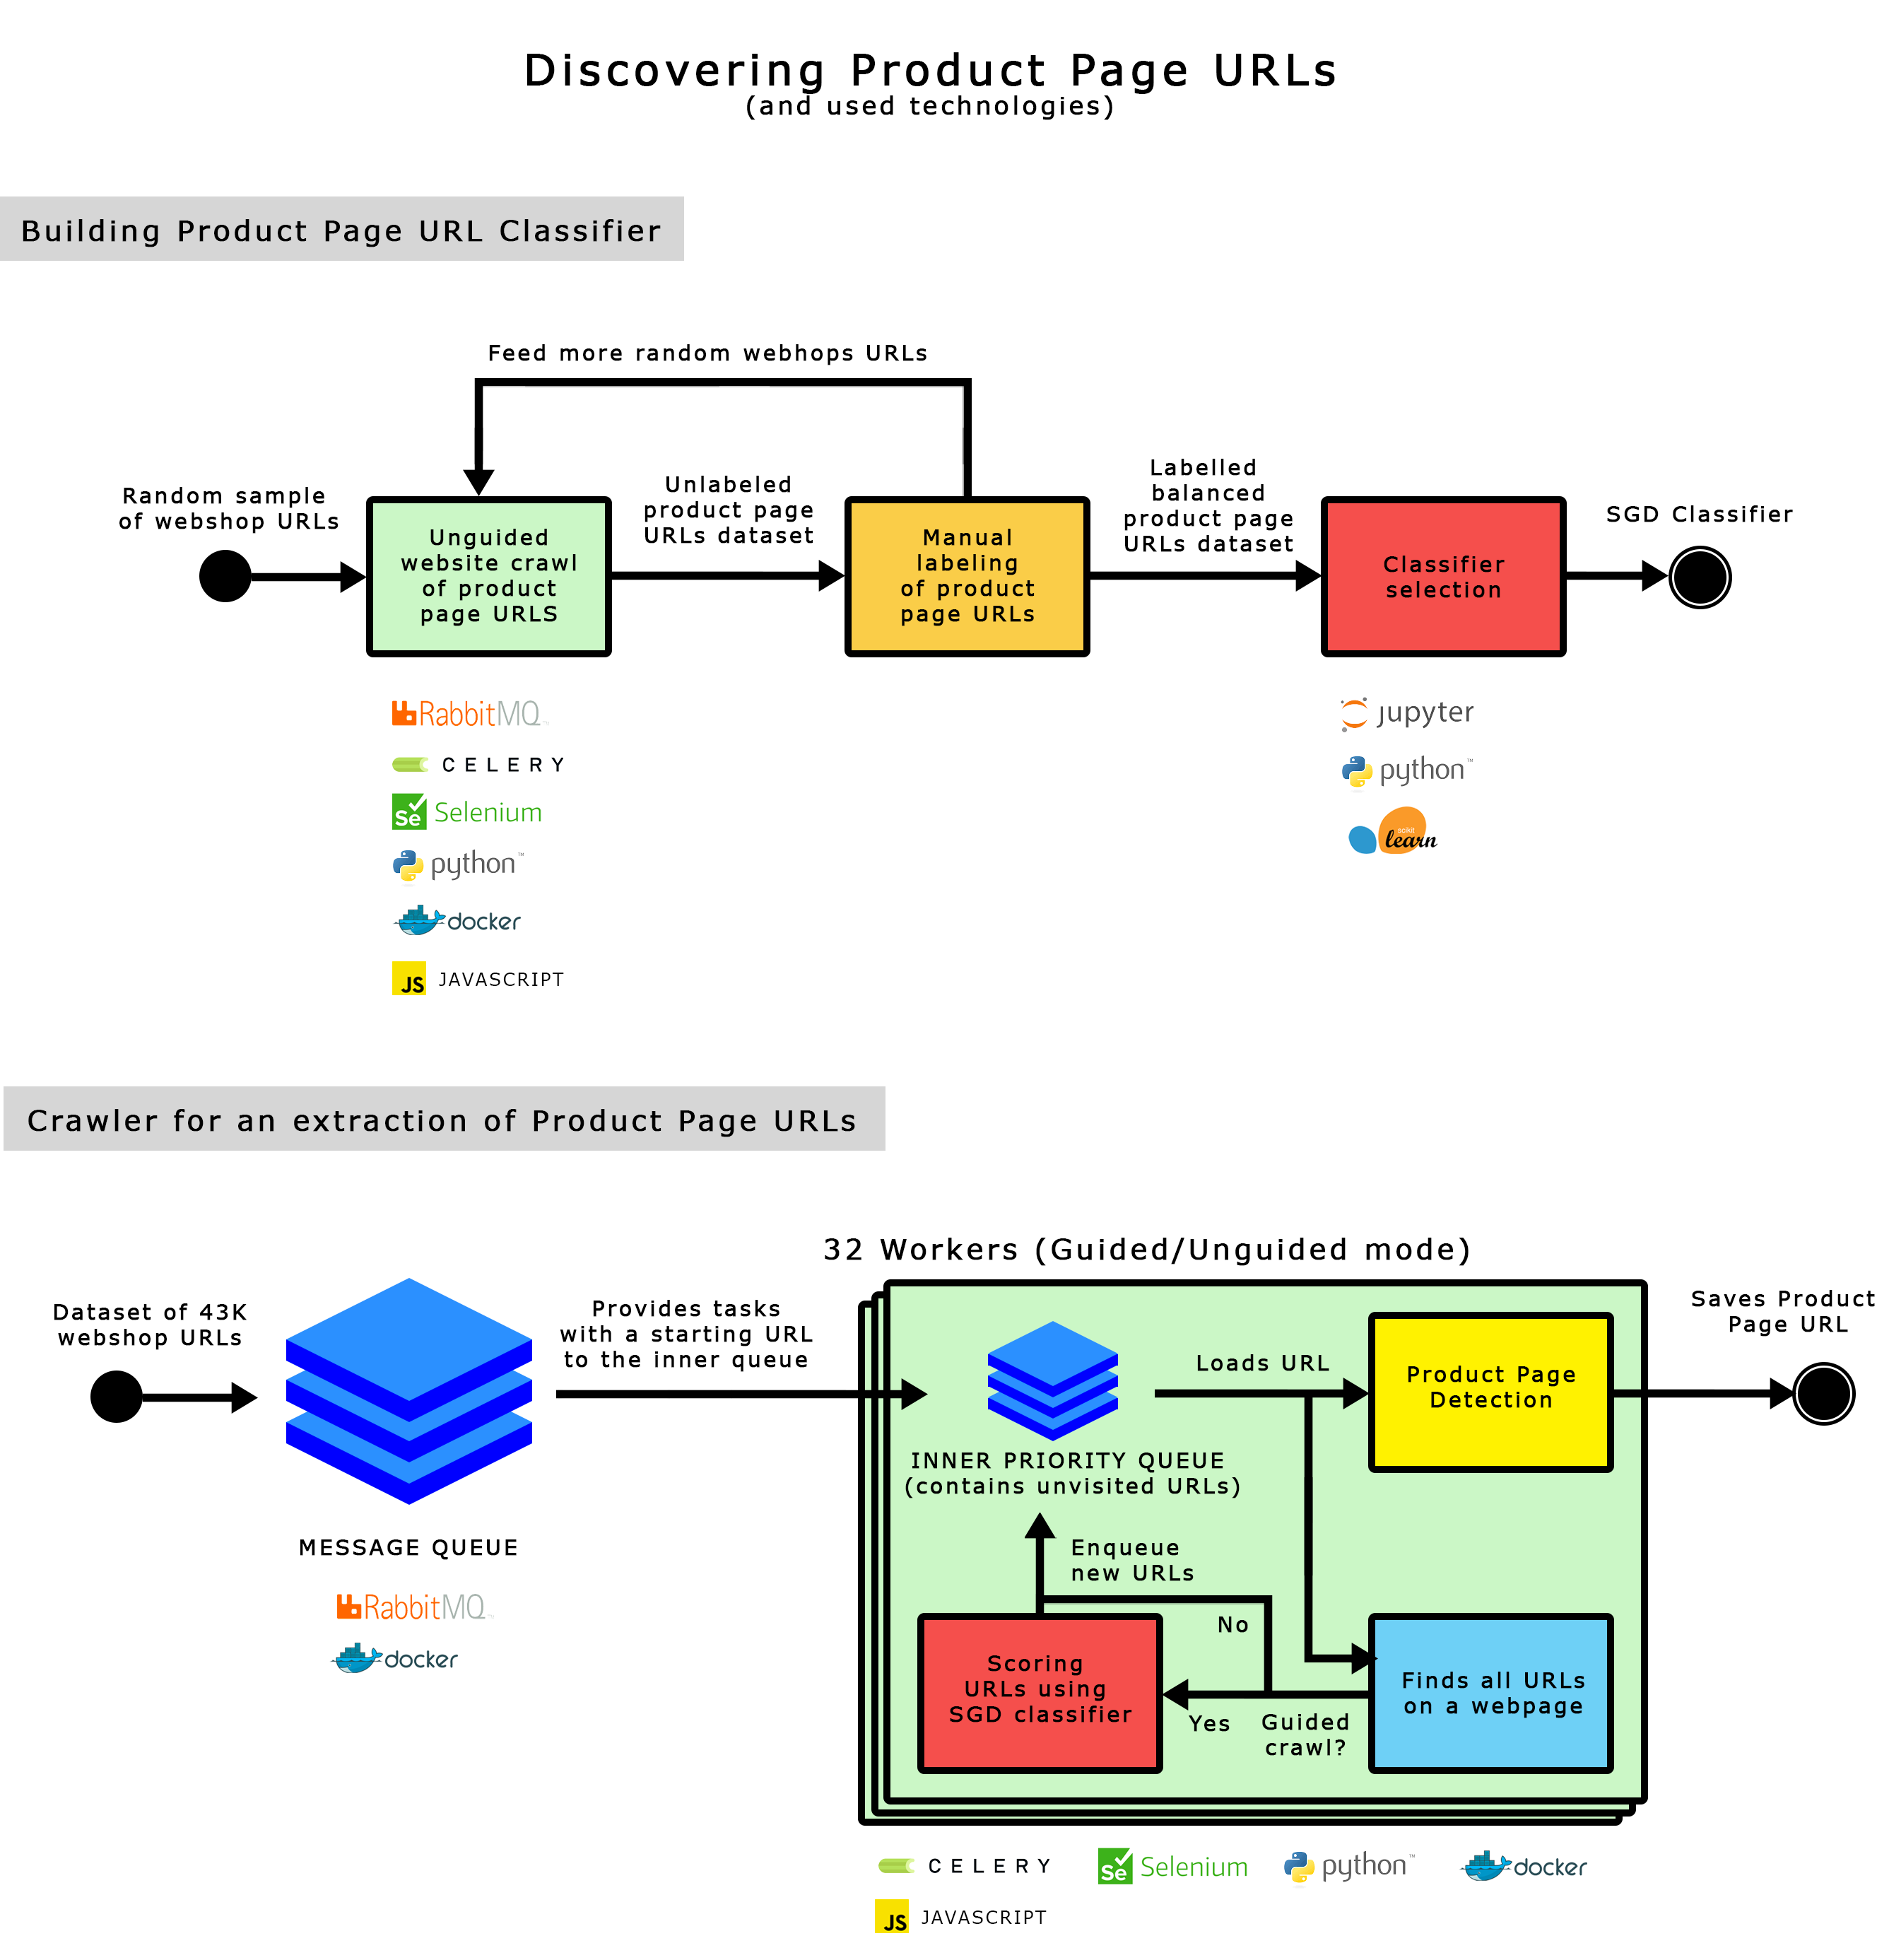
\includegraphics[width=1\linewidth]{media/data_collection.png}
            \caption{The workflow of discovering product page URLs. The crawler can be run in an unguided or a guided mode. The unguided crawl extracts Product Page URLs from a fraction of all Czech webshops. The output is manually labelled and creates a training dataset for the classification model. Further, this model guides the crawler with prioritizing possible Product Page URLs in its inner queue. Therefore, the crawling of a single page is rapidly speeded up.}
            \label{fig:data_collection}
        \end{figure}

        \subsection{Product Page Detection}
        \label{section:product-page-detection}
        A page is classified as a product page if its HTML code contains only one "Add to Cart" button. The detection of such a button is more complicated than it may seem. The researchers implemented complex scoring functions for the detection of such buttons. This includes that the candidates for the "Add to Cart" button are scored not only by the presence of the possible "Add to Cart" phrase (defined in a form of a regular expression) in the inner text or in its attributes but also by the button's size and a contrast ratio of button's colour to the background colour of a body HTML element. To add support for the Czech language, a sample of 50 pages needed to be analysed for the use of "Add to Cart" phrases (see table\ref{table:add-to-cart-phrases}). This analysis led to a modification of the used regular expression.

        \begin{table}[h!]
            \bgroup
            \def\arraystretch{1.65}
            \centering
            \begin{tabular}{l | c} 
                \toprule
                \textbf{Phrase} & \textbf{\#} \\ [0.5ex] 
                \hline
                Do košíku & 19 \\ \hline
                Přidat do košíku & 18 \\ \hline
                Koupit & 7 \\ \hline
                Vložit do košíku & 6 \\ [1ex] 
            \end{tabular}
            \egroup
            \caption{"Add to Cart" phrases in the Czech language found on a random sample of 50 Czech webshops.}
            \label{table:add-to-cart-phrases}
        \end{table}

        \subsection{Unguided Crawl}

        The original classifier distinguishes product page URLs from non-product page URLs that are from English websites. The classifier was trained on a dataset of Czech URLs. This dataset was obtained by running the crawler on a random sample of 100 webshops (mentioned at the beginning of this chapter). The crawler was run to select random URLs to visit while spidering the website instead of predicting which URL was more likely to be a product page. In this random crawl, the crawler's detection marked 398 pages to be product pages. These pages were manually examined, and 308 were actual product pages (77\% accuracy for a random crawl). Additional URLs (not marked as product pages) were iteratively added to the dataset and manually examined. Multiple iterations of additions and examination led to a balanced dataset of 377 product pages and 334 non-product pages.

        \subsection{Product page URL Classifier}

        The classifier is trained in a separate Jupyter Notebook, and it is a modified version of the notebook published by the researchers. This notebook differs from the original notebook in used feature variables, where it adds Czech equivalents to boolean features, representing a specific word in the URL, such as "category" and "product". The Czech counterparts are "kategorie" and "produkt". Czech webshops often use a word "detail" in their URL, which was added as another boolean feature. The last added feature represents whether or not the URL contains a product ID. The rest of original features are a length of the URL, a number of hyphens and slashes and the longest number in the URL. 

        The dataset was split where 90\% records are used for training and 10\% for five-fold cross-validation. Tested classifiers were sklearn's Logistic Regression using L-BFGS solver\cite{logistic-sklearn} and Logistic Regression with Stochastic Gradient Descent learning \cite{sgd-sklearn}. Both classifiers had very similar results on average, but Stochastic Gradient Descent with 78 \% accuracy was chosen as a classifier for the crawler because of its higher validation score (0.83 to 0.76).

        However, none of the added feature variables significantly led to an increased accuracy compared to the original features.

        \subsection{Guided Crawl}

        Once the classifier was trained, the second crawl guided by this classifier was done on the full dataset of \textbf{46,023} webshops' URLs. The classifier helps the crawler to rank URLs on the page by likelihood of being product page URLs. The researchers set certain limits for the crawler from their observations, followed in this part as well. The crawler visits 100 pages or spends 15 minutes at maximum on a single website. It does not visit the same page more than two times. The crawling of a single website can be skipped if the crawler has already found five product pages.

        A total number of 32 workers finished the crawling in 2 days, 7 hours, 20 minutes. During the crawling, \textbf{1,944,980} pages were visited from which \textbf{159,768} were identified as product page URLs on \textbf{43,411} different webshops. The remaining \textbf{2,612} pages were no longer accessible, redirected to a different domain or identified as not being in the Czech language.

    \section{Discovering Textual Segments}
        Since the guided crawl took a significant amount of time to complete, it was assumed that the crawler simulating purchase flow would take even more time to complete due to its higher complexity. During the manual browsing in the previous steps, it was found that the dataset of Czech webshops also contains websites that do not allow consumers to directly buy goods and they just present goods. Obviously, the crawler cannot find product pages on such websites. 

        It can also be assumed that the smaller businesses do not have the funding for their own e-commerce software solution. Because of this, the vast majority of them use third-party solutions. These third-party solutions exhibit the same characteristics, and it cannot be expected from them to contain unique instances of dark patterns across multiple websites. 
        
        For these reasons, only the first \textbf{10K} domains were selected from the list of \textbf{43,411} e-shops for the following crawling step. Ten thousand different domains are also comparable to the number of domains used by the Princeton researchers---i.e. 11,286 unique domains. The filtering of the list of given product URLs by domain name returned \textbf{33,782} product URLs.
        
        The crawler used in this part of the study is almost identical to the crawler (in their study referred to as Checkout crawler) published by the Princeton researchers.

        The crawler performs two concurrent tasks. It is \nameref{section:flow-simulation} and \nameref{section:text-extraction}. The workflow of this crawler is shown in Figure\ref{fig:data_collection2}

        \begin{figure}[ht]
            \centering
            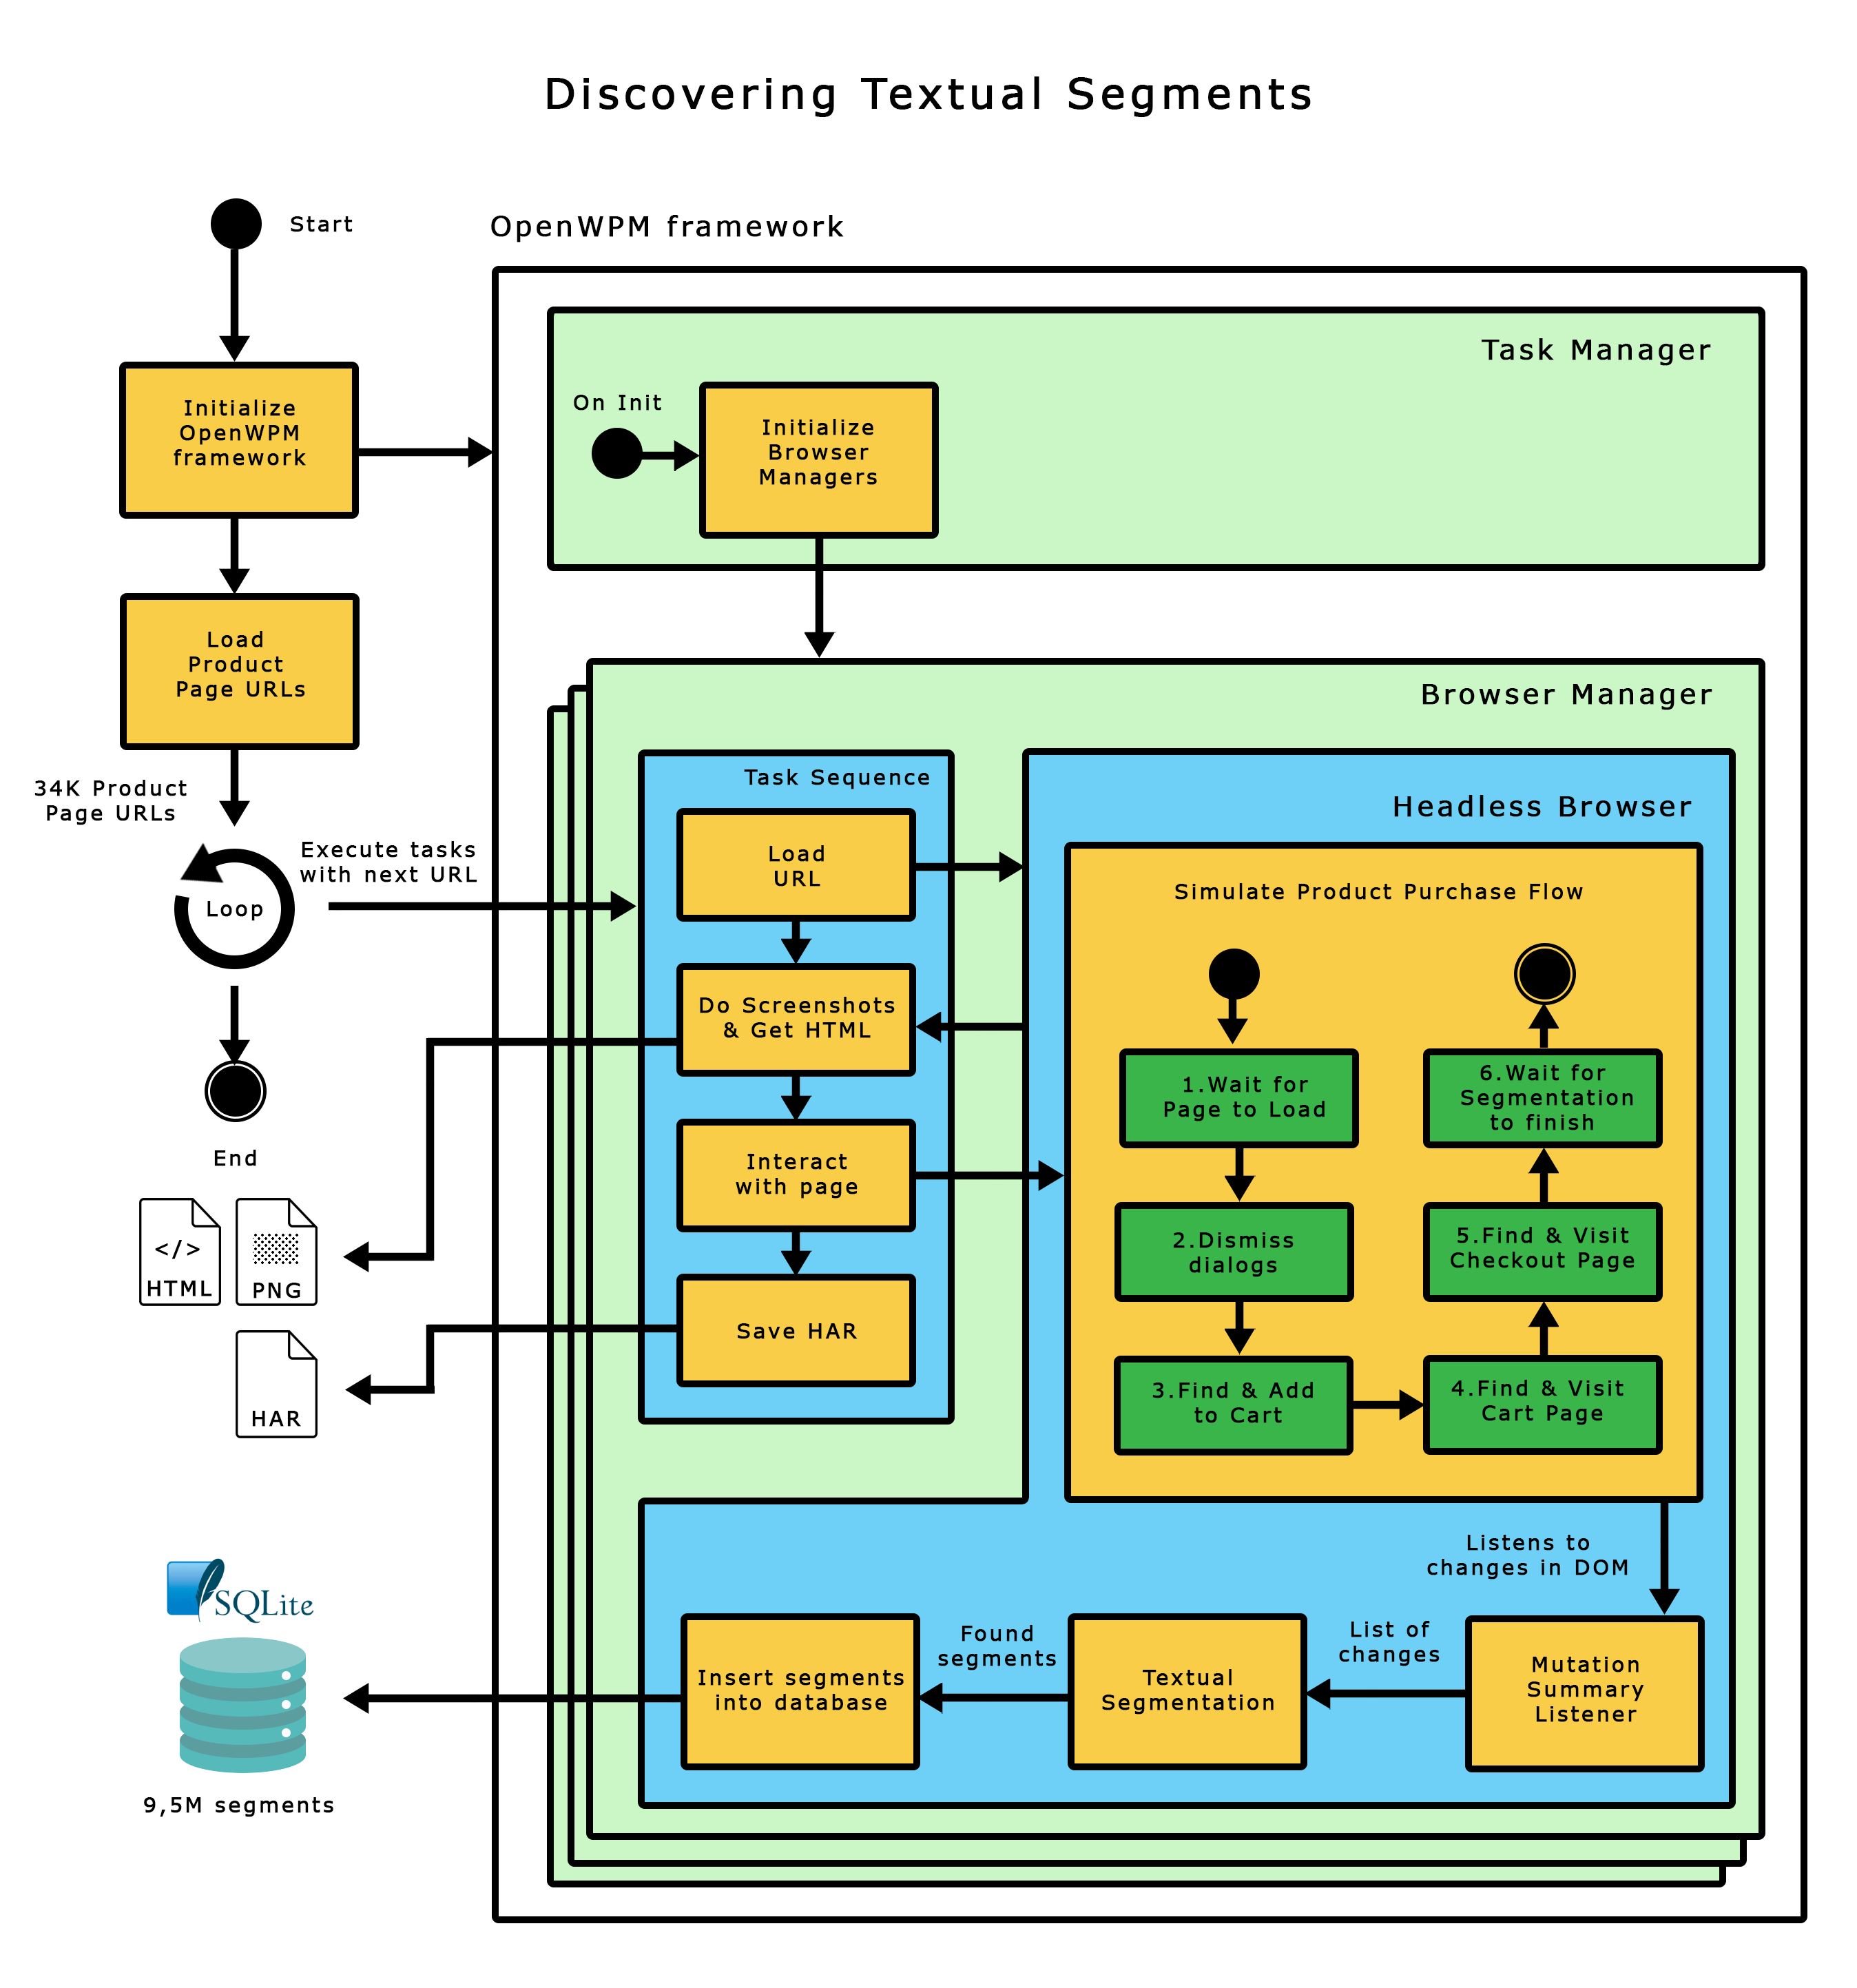
\includegraphics[width=1\linewidth]{media/data_collection2.png}
            \caption{The workflow of discovering textual segments from the dataset of Product page URLs. OpenWPM framework creates multiple workers (Browser Managers) and serves them a sequence of tasks they follow. The task manager is capable of orchestrating the workers, that finished previous tasks and are ready for crawling a Product Page URL.}
            \label{fig:data_collection2}
        \end{figure}

        \subsection{Product Purchase Flow Simulation}
        \label{section:flow-simulation}
            By analyzing the code for the simulation, it was found that the crawling logic can remain the same because it is independent of the language used. Nevertheless, the original crawler does not support the Czech language. This is crucial in searching appropriate buttons for interactions with web pages. The modified crawler adds Czech language support.

            It contains modified regular expressions that are used by scoring functions. The scoring functions are very similar to the one already described in Section \ref{section:product-page-detection}. These functions allow the crawler to find the buttons on the website. Because of that, the crawler can run independently on many websites with different designs. 

            The crawler is able to handle edge cases to simulate user interaction, such as dismissing pop-up dialogues and identifying interfaces for selecting product attributes. Also, the crawler takes a screenshot every second and saves only the screenshots that differ in base64 form \cite{base64} from a previously taken screenshot. The whole communication, every interaction is saved in HTTP Archive (HAR) but is omitted from the analysis done in this thesis.
            
            The product purchase flow consists of four steps:

        \subsubsection{Adding Product to Cart}
            Firstly, the crawler searches the interface for selecting product variants and selects one of them. This is not a very complex algorithm. It searches for every select HTML element on the page, and the crawler tries to set it to a random value. This was not modified from the original crawler because it is not dependent on the used language. After that, the crawler searches for the "Add to Cart" button. The regular expression defining the possible values was modified to support Czech languages, which is made and described earlier in the section \ref{section:product-page-detection}. Once the button is found, the crawler clicks it to add the product to the cart.

        \subsubsection{Searching View Cart}
            Secondly, the crawler searches for a "View Cart" button in a similar way as it searches for the "Add to Cart" button. The regular expression defining the possible phrases was also modified to support Czech equivalents of "View Cart" and its synonyms. Results from the analysis of one hundred websites have shown that one hundred per cent of Czech e-shops uses the word "košík" (or its declination).


        \subsubsection{Searching Checkout Button}
            Thirdly, once the product is added to the cart, the crawler locates a button that leads to the final Checkout page.

            On a random sample of one hundred product URLs, the following keywords from phrases used to proceed to the Checkout page were found:

            \begin{table}[h!]
                \centering
                \bgroup
                \def\arraystretch{1.65}
                \begin{tabular}{l | c | l | c} 
                    \toprule
                    \textbf{Phrase} & \textbf{\#} & \textbf{Phrase} & \textbf{\#} \\ \hline
                    Pokračovat & 51 & Pokladna & 7  \\ \hline
                    Objednávka & 25 & Přejít & 6 \\ \hline
                    Doprava & 14 & Objednat & 5 \\ \hline
                    Platba & 13 & Dále & 1 \\ \hline
                \end{tabular}
                \egroup
                \caption{Most common Czech words inside buttons that proceed to the Checkout page. Occurrences were found on a random sample of one hundred Czech webshops.}
                \label{table:add-to-cart-phrases}
            \end{table}

        \subsubsection{Waiting on Checkout Page}
            The crawler does no interaction on the checkout page. It only waits 10 seconds, so the page segmentation defined below has enough time to finish.

        \subsection{Text Extraction using Page Segmentation}
        \label{section:text-extraction}
        Since the page segmentation is language-independent, it is used in its original form as it was published by the researchers. 
        
        While crawling the website, the crawler extracts page segments of every visited page and from every change that can occur during the crawl. Researchers describe page segments as building blocks of a website, representing smaller sections. These segments shape a dataset later used in the data analysis and clustering. Researchers define\cite{dark-patterns-at-scale} a single page segment as a visible HTML element that does not contain block-level element\cite{block-element} and contains at least one text element\cite{text-element}. 
        
        The crawler waits for the web page to load completely before the page segmentation starts. Even after the complete loading of the web page, the browser can render additional content into the DOM. The user's interaction may trigger these changes in the web page, or pop-up windows may appear. To capture all these changes, researchers integrated Mutation Summary \cite{mutation-summary} library into the crawler. This library observes changes in the DOM and emits events that retrieve all the changes in a form of an array, which is again processed by the page segmentation.

        The researchers included a pseudocode of the page segmentation algorithm and an illustration of the algorithm's output in their work\cite{dark-patterns-at-scale}.

        Each segment is stored as one record in the SQLite database, where each document contains the segment's HTML Element type, innerText, dimensions, coordinates on the page and styles (CSS colour and background-color).

        From the crawling of the \textbf{10K} Czech webshops, the crawler visited \textbf{33,782} web pages, where it captured \textbf{~9,5M} segments. It can be said that this number of captured segments corresponds to the number of segments the Princeton researchers extracted from the same number of web pages. They extracted over 13M segments from 53K web pages.
